%%%%%%%%%%%%%%%%%%%%%%%%%%%%%%%%%%%%%%%%%
% Lachaise Assignment
% LaTeX Template
% Version 1.0 (26/6/2018)
%
% This template originates from:
% http://www.LaTeXTemplates.com
%
% Authors:
% Marion Lachaise & François Févotte
% Vel (vel@LaTeXTemplates.com)
%
% License:
% CC BY-NC-SA 3.0 (http://creativecommons.org/licenses/by-nc-sa/3.0/)
% 
%%%%%%%%%%%%%%%%%%%%%%%%%%%%%%%%%%%%%%%%%

%----------------------------------------------------------------------------------------
%	PACKAGES AND OTHER DOCUMENT CONFIGURATIONS
%----------------------------------------------------------------------------------------

\documentclass{article}

%%%%%%%%%%%%%%%%%%%%%%%%%%%%%%%%%%%%%%%%%
% Lachaise Assignment
% Structure Specification File
% Version 1.0 (26/6/2018)
%
% This template originates from:
% http://www.LaTeXTemplates.com
%
% Authors:
% Marion Lachaise & François Févotte
% Vel (vel@LaTeXTemplates.com)
%
% License:
% CC BY-NC-SA 3.0 (http://creativecommons.org/licenses/by-nc-sa/3.0/)
% 
%%%%%%%%%%%%%%%%%%%%%%%%%%%%%%%%%%%%%%%%%

%----------------------------------------------------------------------------------------
%	PACKAGES AND OTHER DOCUMENT CONFIGURATIONS
%----------------------------------------------------------------------------------------

\usepackage{amsmath,amsfonts,stmaryrd,amssymb} % Math packages

\usepackage{enumerate} % Custom item numbers for enumerations

\usepackage[ruled]{algorithm2e} % Algorithms

\usepackage[framemethod=tikz]{mdframed} % Allows defining custom boxed/framed environments

\usepackage{listings} % File listings, with syntax highlighting
\lstset{
	basicstyle=\ttfamily, % Typeset listings in monospace font
}

%----------------------------------------------------------------------------------------
%	DOCUMENT MARGINS
%----------------------------------------------------------------------------------------

\usepackage{geometry} % Required for adjusting page dimensions and margins

\geometry{
	paper=a4paper, % Paper size, change to letterpaper for US letter size
	top=2.5cm, % Top margin
	bottom=3cm, % Bottom margin
	left=2.5cm, % Left margin
	right=2.5cm, % Right margin
	headheight=14pt, % Header height
	footskip=1.5cm, % Space from the bottom margin to the baseline of the footer
	headsep=1.2cm, % Space from the top margin to the baseline of the header
	%showframe, % Uncomment to show how the type block is set on the page
}

%----------------------------------------------------------------------------------------
%	FONTS
%----------------------------------------------------------------------------------------

\usepackage[utf8]{inputenc} % Required for inputting international characters
\usepackage[T1]{fontenc} % Output font encoding for international characters
\usepackage[babel]{} % Output font encoding for international characters

\usepackage{XCharter} % Use the XCharter fonts

%----------------------------------------------------------------------------------------
%	COMMAND LINE ENVIRONMENT
%----------------------------------------------------------------------------------------

% Usage:
% \begin{commandline}
%	\begin{verbatim}
%		$ ls
%		
%		Applications	Desktop	...
%	\end{verbatim}
% \end{commandline}

\mdfdefinestyle{commandline}{
	leftmargin=10pt,
	rightmargin=10pt,
	innerleftmargin=15pt,
	middlelinecolor=black!50!white,
	middlelinewidth=2pt,
	frametitlerule=false,
	backgroundcolor=black!5!white,
	frametitle={Command Line},
	frametitlefont={\normalfont\sffamily\color{white}\hspace{-1em}},
	frametitlebackgroundcolor=black!50!white,
	nobreak,
}

% Define a custom environment for command-line snapshots
\newenvironment{commandline}{
	\medskip
	\begin{mdframed}[style=commandline]
}{
	\end{mdframed}
	\medskip
}

%----------------------------------------------------------------------------------------
%	FILE CONTENTS ENVIRONMENT
%----------------------------------------------------------------------------------------

% Usage:
% \begin{file}[optional filename, defaults to "File"]
%	File contents, for example, with a listings environment
% \end{file}

\mdfdefinestyle{file}{
	innertopmargin=1.6\baselineskip,
	innerbottommargin=0.8\baselineskip,
	topline=false, bottomline=false,
	leftline=false, rightline=false,
	leftmargin=2cm,
	rightmargin=2cm,
	singleextra={%
		\draw[fill=black!10!white](P)++(0,-1.2em)rectangle(P-|O);
		\node[anchor=north west]
		at(P-|O){\ttfamily\mdfilename};
		%
		\def\l{3em}
		\draw(O-|P)++(-\l,0)--++(\l,\l)--(P)--(P-|O)--(O)--cycle;
		\draw(O-|P)++(-\l,0)--++(0,\l)--++(\l,0);
	},
	nobreak,
}

% Define a custom environment for file contents
\newenvironment{file}[1][File]{ % Set the default filename to "File"
	\medskip
	\newcommand{\mdfilename}{#1}
	\begin{mdframed}[style=file]
}{
	\end{mdframed}
	\medskip
}

%----------------------------------------------------------------------------------------
%	NUMBERED QUESTIONS ENVIRONMENT
%----------------------------------------------------------------------------------------

% Usage:
% \begin{question}[optional title]
%	Question contents
% \end{question}

\mdfdefinestyle{question}{
	innertopmargin=1.2\baselineskip,
	innerbottommargin=0.8\baselineskip,
	roundcorner=5pt,
	nobreak,
	singleextra={%
		\draw(P-|O)node[xshift=1em,anchor=west,fill=white,draw,rounded corners=5pt]{%
		Question \theQuestion\questionTitle};
	},
}

\newcounter{Question} % Stores the current question number that gets iterated with each new question

% Define a custom environment for numbered questions
\newenvironment{question}[1][\unskip]{
	\bigskip
	\stepcounter{Question}
	\newcommand{\questionTitle}{~#1}
	\begin{mdframed}[style=question]
}{
	\end{mdframed}
	\medskip
}

%----------------------------------------------------------------------------------------
%	WARNING TEXT ENVIRONMENT
%----------------------------------------------------------------------------------------

% Usage:
% \begin{warn}[optional title, defaults to "Warning:"]
%	Contents
% \end{warn}

\mdfdefinestyle{warning}{
	topline=false, bottomline=false,
	leftline=false, rightline=false,
	nobreak,
	singleextra={%
		\draw(P-|O)++(-0.5em,0)node(tmp1){};
		\draw(P-|O)++(0.5em,0)node(tmp2){};
		\fill[black,rotate around={45:(P-|O)}](tmp1)rectangle(tmp2);
		\node at(P-|O){\color{white}\scriptsize\bf !};
		\draw[very thick](P-|O)++(0,-1em)--(O);%--(O-|P);
	}
}

% Define a custom environment for warning text
\newenvironment{warn}[1][Warning:]{ % Set the default warning to "Warning:"
	\medskip
	\begin{mdframed}[style=warning]
		\noindent{\textbf{#1}}
}{
	\end{mdframed}
}

%----------------------------------------------------------------------------------------
%	INFORMATION ENVIRONMENT
%----------------------------------------------------------------------------------------

% Usage:
% \begin{info}[optional title, defaults to "Info:"]
% 	contents
% 	\end{info}

\mdfdefinestyle{info}{%
	topline=false, bottomline=false,
	leftline=false, rightline=false,
	nobreak,
	singleextra={%
		\fill[black](P-|O)circle[radius=0.4em];
		\node at(P-|O){\color{white}\scriptsize\bf i};
		\draw[very thick](P-|O)++(0,-0.8em)--(O);%--(O-|P);
	}
}

% Define a custom environment for information
\newenvironment{info}[1][Info:]{ % Set the default title to "Info:"
	\medskip
	\begin{mdframed}[style=info]
		\noindent{\textbf{#1}}
}{
	\end{mdframed}
}
 % Include the file specifying the document structure and custom commands

%----------------------------------------------------------------------------------------
%	ASSIGNMENT INFORMATION
%----------------------------------------------------------------------------------------

\title{MAE001: Modelagem Matemática em Finanças I} % Title of the assignment

\author{Ramon Duarte de Melo\\ \texttt{ramonduarte@poli.ufrj.br}} % Author name and email address

\date{Universidade Federal do Rio de Janeiro (UFRJ) --- \today} % University, school and/or department name(s) and a date

%----------------------------------------------------------------------------------------

\begin{document}

\maketitle % Print the title

%----------------------------------------------------------------------------------------
%	INTRODUCTION
%----------------------------------------------------------------------------------------

\section*{Introdução} % Unnumbered section

O objetivo do Projeto I é implementar, avaliar e comparar o algoritmo recursivo proposto pelo livro no capítulo 1.3 e o Método de Monte-Carlo, aplicados à determinação do valor de contratos americanos e europeus de opção de compra e venda, realizando comparações de cunho matemático-estatístico e produzindo gráficos com tais observações. 

Para tal, foi utilizada a linguagem \emph{Python 3.6.7}, com os módulos \emph{numpy} (métodos numéricos) e \emph{matplotlib.pyplot} (visualização de dados).
O programa requer a instalação destes módulos, mas possui uma ferramenta de instalação automatizada das dependências (\emph{pipenv}). 

O código utilizado neste trabalho, bem como o deste relatório e as imagens geradas, foi aberto e disponibilizado publicamente no repositório https://github.com/ramonduarte/mmftrab2.


%----------------------------------------------------------------------------------------
%	PROBLEM 1
%----------------------------------------------------------------------------------------

\section*{Atividade 1} % Numbered section

Nesta atividade, foi implementado o algoritmo sugerido no livro em seu capítulo 1.3.
O procedimento é composto de três etapas:

\begin{enumerate}
	\item obtenção dos valores finais, com especial atenção para evitar a explosão combinatória típica do modelo binomial.
	\item cálculo recursivo dos valores intermediários utilizando os valores finais.
	\item dedução do valor inicial $V_{0}$ do contrato, que também representa seu custo pela teoria de precificação da arbitragem.
\end{enumerate}

Os contratos escolhidos possuem os mesmos parâmetros, tanto para a opção de compra, quanto para a opção de venda:

\begin{itemize}
	\item valor inicial do ativo: 4
	\item taxa de valorização: 100%
	\item taxa de desvalorização: 50%
	\item taxa de renda fixa: 25%
	\item preço de \emph{strike}: 5
\end{itemize}

Estes parâmetros foramutilizados junto às probabilidades neutras a risco $\tilde{p} = \tilde{q} = 0.5$.
Foram calculados os valores para 10 simulações, tais que $N = 2^{k}; k = 1, 2, ..., 10$.


\begin{figure}[]
	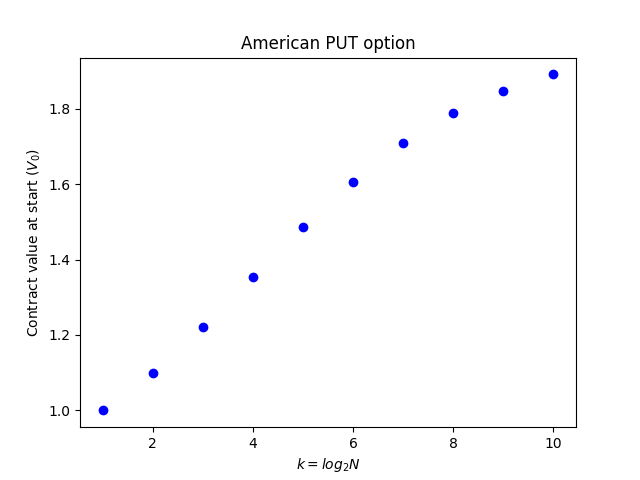
\includegraphics[width=\linewidth*9/10]{Figure_0.png}
	\centering
	
	\label{}
\end{figure}


\begin{figure}[]
	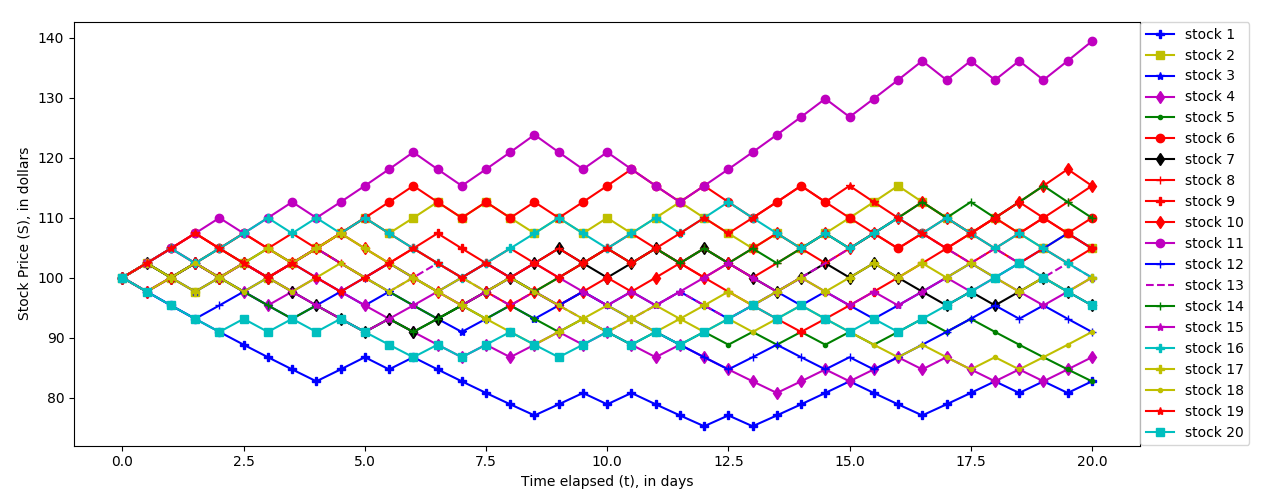
\includegraphics[width=\linewidth*9/10]{Figure_1.png}
	\centering
	
	\label{}
\end{figure}

Opções de venda (PUT) têm sua valorização limitada pelo fato de que dependem da queda do valor do ativo.
Tipicamente, ativos costumam possuir um piso finito, abaixo do qual seu preço não pode cair (neste exemplo, zero).
Porém, o crescimento é linear no início da curva, até $k = 8$, aproximadamente. 

Opções de compra (CALL), por outro lado, possuem crescimento ilimitado.
O crescimento é exponencial mesmo utilizando uma base maior ($10$) para o valor inicial do contrato que para o tempo ($k = log_{2} \ N$ neste cenário).



%----------------------------------------------------------------------------------------
%	PROBLEM 2
%----------------------------------------------------------------------------------------


\section*{Atividade 2}

Os mesmos contratos da atividade anterior foram recalculados utilizando o Método de Montecarlo.
Desta vez, as três etapas são:

\begin{enumerate}
	\item produção dos caminhos a serem percorridos dentro da árvore de possibilidades.
	\item determinação do valor do contrato para cada caminho (repetido $M$ vezes).
	\item cálculo da média dos valores encontrados.
\end{enumerate}

Este método produz resultados estimados, ao passo que o anterior produz resultados tidos como exatos.
Por isto, para esta atividade, foi fixado o valor de $M=5000$, repetidos os contratos anteriores e comparados os resultados.
A métrica utilizada foi o erro quadrático médio, para evitar que erros simétricos se anulem.

Os contratos de venda tiveram alta variância no erro quadrático médio, indicando que, se existe, a influência da extensão do prazo (ou redução do intervalo de discretização do tempo) é pequena.

Os contratos de compra, por outro lado, tiveram crescimento exponencial similar ao do próprio valor inicial do contrato.

\begin{figure}[H]
	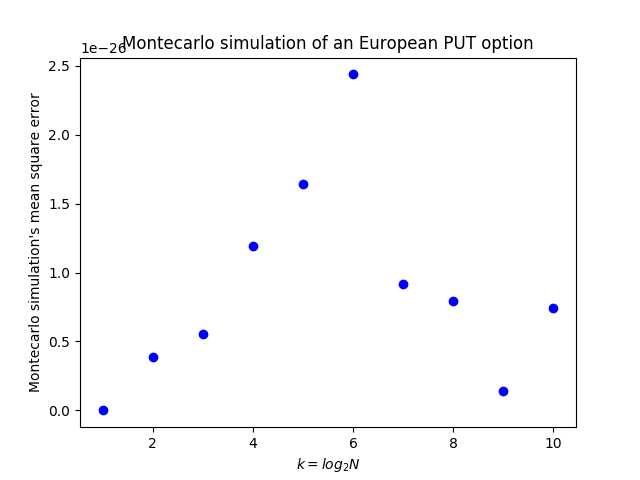
\includegraphics[width=\linewidth]{Figure_2.png}
	\centering
	
	\label{}
\end{figure}

\begin{figure}[H]
	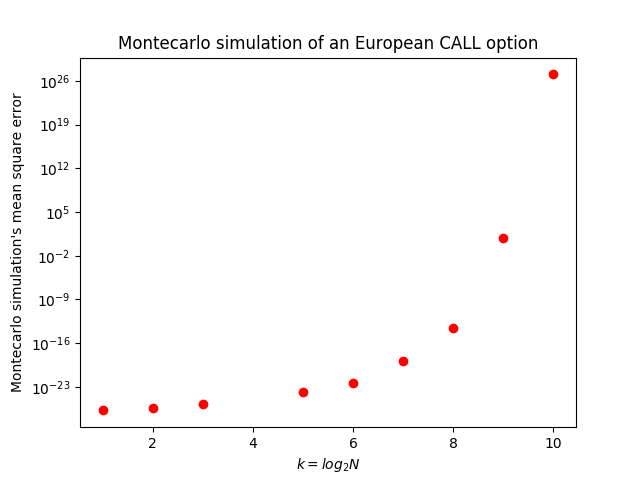
\includegraphics[width=\linewidth]{Figure_3.png}
	\centering
	
	\label{}
\end{figure}

%----------------------------------------------------------------------------------------
%	PROBLEM 2
%----------------------------------------------------------------------------------------

\section*{Atividade 3}

Por fim, para esta atividade, foi escolhido o contrato europeu de compra com \emph{lookback}, descrito na página 17 do livro.
A principal diferença para um contrato europeu de compra regular é a função do valor do contrato:

\begin{equation}
	V_{n} = \max_{0 \leq j \leq n} S_{j}  -  K
\end{equation}

Os valores são idênticos ao contrato anterior, exceto pelo preço de strike $K = 0$.
A dependência do caminho está estabelecida pela necessidade de guardar o maior valor que o ativo atingiu previamente.

O \emph{lookback} provê um piso mais elevado ao contrato de opção e, por isso, o crescimento exponencial é observado novamente.
Os valores iniciais do são ainda mais elevados nesta modalidade.

No livro, os autores utilizam o algoritmo da seção 1.3 (o mesmo usado na Atividade 1), porém os tempos são significativamente mais curtos. Para $k \in [1, 2]$, os resultados foram compatíveis. 

\begin{figure}[H]
	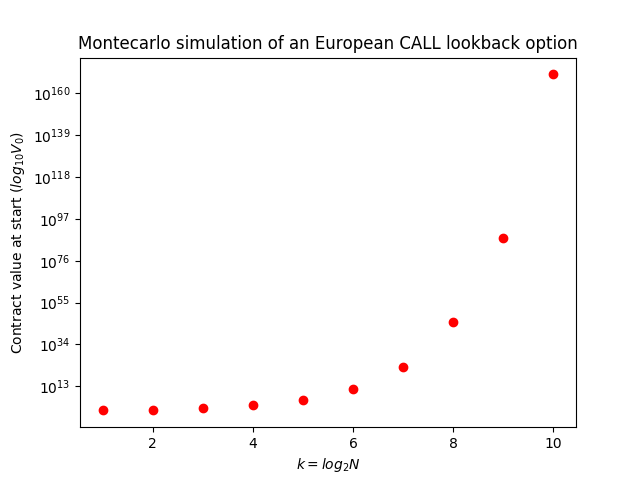
\includegraphics[width=\linewidth]{Figure_5.png}
	\centering
	
	\label{}
\end{figure}



\end{document}
